% !TEX TS-program = pdflatex
% !TEX encoding = UTF-8 Unicode

% An alternative to the standard LaTeX letter class.

\documentclass[fontsize=12pt, paper=a4]{scrbook}
\makeatletter\@addtoreset{chapter}{part}\makeatother%

% Don't forget to read the KOMA-Script documentation, scrguien.pdf

\usepackage[utf8]{inputenc}

\setcounter{secnumdepth}{4}

\usepackage{amssymb}

%
\usepackage{float}

% tikz
\usepackage{tikz}
\usetikzlibrary{trees}

% listings
\usepackage{minted}

\newcommand\relativepath{}
\newcommand\relative[1]{\relativepath#1}

\newcommand\pod{POD}
\newcommand\awsc{AWS console}
\newcommand\aws{AWS}
\newcommand\vadorc[1]{VADORC#1}
\newcommand\rdp{RDP}
\newcommand\awsstddevkey{Dev-US-East-1}
\newcommand\rootuser{\emph{root}}
\newcommand\git{git}
\newcommand\axceleratepod{AxceleratePod}
\newcommand\dockerfile{Dockerfile}

% minted
\setminted[yaml]{linenos,frame=single,labelposition=bottomline}
\setminted[text]{linenos,frame=single,labelposition=bottomline}

\begin{document}
	\tableofcontents
	\renewcommand\relativepath{part_00/}
	\part{Introduction}
	\chapter{Goals of this documentation}
	% Not nice!! We need a solution to overcome this drawback!
	\renewcommand\relativepath{c:/documentation/recomlinarch/part_01/}
	\part{The Linux architecture in the AWS environment}
	\chapter{The build-to-deployment pipeline}
% Describe the hole pipeline (code -> jenkins -> docker repos + cg + ami etc.) + picture
	\chapter{The Linux host environment}
Before an engine can start up several configurations need to take place. Some of those configurations are made on the Linux host side and some
within the engine docker container. In any case the bootloader is the instance which is responsible to setup the environment and put it in a well
defined state such that the engine can function properly.
	\section{Filesystem layout of the Linux host}\label{p01:ch021}
	The filesystem layout is oriented on the filesystem hierarchy standard (FHS). In \emph{/srv} we find the following hierarchy:
	
	\tikzstyle{every node}=[draw=black,thick,anchor=west]
	\tikzstyle{selected}=[draw=red,fill=red!30]
	\tikzstyle{optional}=[dashed,fill=gray!50]
	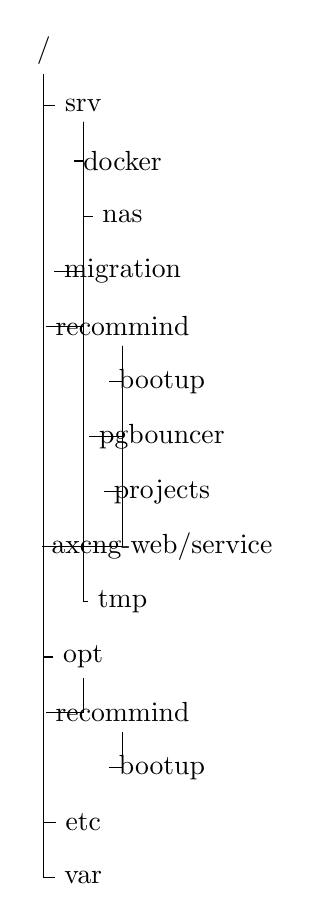
\begin{tikzpicture}[
		grow via three points={one child at (0.5,-0.7) and two children at (0.5,-0.7) and (0.5,-1.4)},
		edge from parent path={(\tikzparentnode.south) |- (\tikzchildnode.west)}]
		\node(root) {/}
			child { node {srv}
				child { node {docker}}
				child { node {nas}}
				child { node {migration}}
				child { node {recommind}
					child { node {bootup}}
					child { node {pgbouncer}}
					child { node {projects}}
					child { node {axcng-web/service}}
				}
				child [missing] {}
				child [missing] {}
				child [missing] {}
				child [missing] {}
				child { node {tmp}}
			}
			child [missing] {}
			child [missing] {}
			child [missing] {}
			child [missing] {}
			child [missing] {}
			child [missing] {}
			child [missing] {}
			child [missing] {}
			child [missing] {}
			child { node {opt}
				child { node {recommind}
					child { node {bootup}}
				}
			}
			child [missing] {}
			child [missing] {}
			child { node {etc}}
			child { node {var}};
	\end{tikzpicture}
	
	We omit the presentation of directories which are not touched by us. As already said they follow the FHS. The other directories are maintained by us and contain the following contents.
	\paragraph{/srv:} \emph{/srv} contains data which are persistent by services. In our environment this means:
	\begin{description}
		\item[docker] Here is where the docker service stores the docker images and containers. It is usually not of importantce to us although it might run out of disk if too many docker images and containers are pulled and spawned respectively. However on normal operation the bootloader shutdown scripts take care to remove any container spawned earlier. The bootloader startup scripts in turn take care to spawn new containers as specified in their respective configuration files.
		\item[nas] In every POD a Windows-share server is being instantiated and is used - for instance - to store production or CSV exports. In order to give the engine process access to those server locations the POD specific Windows-share is mounted into this location and mapped into the engine container later on.
		\item[migration] If an engine server is being migrated from the Windows to the Linux environment orchestration takes care about attaching the "old" Windows drives to the Linux instance. If that is the case the bootloader detects the Windows drives and mounts them read-only into this location. The bootloader within the engine container - once started - checks if there is need to migrate the contents on this location to the new one.
		\item[recommind] This is the location where everything is stored by our processes and which is being mapped into the engine container such that the engines do have access to it. The \emph{bootup} subdirectory contains the logfile produced by the bootloader which runs inside the engine container. If the engine container does not come up for what every reason this would be \textbf{the first place} to inspect to get an idea of what possibly went wrong during engine docker bootup. The \emph{pgbouncer} subdirectory is being used by the pgbouncer container for storing its bootup log files. The \emph{projects} directory is our \emph{\$MINDSERVER\_PROJECTS} directory and contains every project plus the launcher service and processcontrol content. On the app-servers the \emph{axcng-web} and \emph{axcng-service} directories are located here too but should usually not of the concern of the index team.
		\item[tmp] First: this location has \textbf{nothing} to do with the temp drive/directory of the Linux host. For engine servers dedicated temp-drives are created and attachted to the engine instance. Those drives are mounted to this location and mapped into the docker container later on to provide a dedicated temp drive large enough to hold every temporary data the engine container comes up with. It is used by the container which is provided by the docker service thus it is located in \emph{/srv}.
	\end{description}
	
	\paragraph{/opt:} contains the software packages which run on the server. The only relervant one for the index team is located in the subdirectory \emph{recommind/bootup} which contains the bootloader which runs on the Linux host instance. Besides the bootloader itself it also contains the bootloader logfile(s) and is therefore the first place to take a look at when the Linux host bootup procedure failed.
	
	\paragraph{/etc:} is the directory containing host specific and system-wide configuration files. Relervant for the index team are here the subdirectories
	\begin{description}
		\item[samba] which contains the samba configuration \emph{smb.conf} and which might be of intereset in case an operator has problems accessing the instances shared volume (which is \emph{/srv/recommind}).
		\item[systemd] which contains the \emph{systemd} unit-description files which specifies the \emph{systemd} endpoints to startup and shutdown recommind services (here shutdown phases of the Linux host bootloader).
	\end{description}
	
	\paragraph{/var:} is the directory containing every variable - i.e. continually changed - files during system uptime. Most relevant for problem analysis is the subdirectory \emph{log} which contains several logfiles especially \emph{syslog} among the others which is the one of the logfiles to inspect if something went wrong during system startup but also during system uptime.
	
	\section{Bootloader system configuration}
	The Linux host instances are being configured by the bootloader in various ways. Here we want to describe every phase in detail but omit the presentation of the phase specific source code. An detailed presentation of the Linux host bootloader source will be treated in chapter \ref{p01:ch04} on page \pageref{p01:ch04}.
	
		\subsection{\emph{bootup} phases}\label{p01:ch221}
			The \emph{bootup} phases will run at every instance startup. It's important that one of the phases creates \emph{systemd} unit-descriptions and places them to \emph{/etc/systemd}. The \emph{systemd} init process in turn ensures that every such unit-description is read and produces a \emph{systemd} service endpoint. It will then show up by the \emph{systemctl} Linux command and can be started, stopped, restarted and queried for its status with that command. When enabled every endpoint is automatically started (in a specified order) by the \emph{systemd} init process at system startup.
			\subsubsection{prestart00}
			This phase is responsible for the following configurations:
			\begin{description}
				\item[Volumes] If a Linux instance is being created by the orchestration several AWS volumes might be created and attached to the instance. For every such volume a description in the bootloader configuration file exists which tells the volume setup code where the volume node is, in which logical volume group it depends and what filesystem it needs to carry.
				\begin{listing}[H]
					\caption{A sample volume description}
					\label{lst:p01:ch01:linhost_vol_desc}
					\inputminted{yaml}{\relative{chapter_01/section_3.2/volume_description_example.yaml}}
				\end{listing}
				This description is a 1:1 mapping as it would appear in the \emph{/etc/fstab} file.
			
				The \emph{block\_device} member tells us whether we're dealing with a block device. It is usually always true in the 			production environment but not necessarily in development or staging. For testing purposes it is possible to not specify this member or set it to \emph{False} and use some regular directory on disk and perform a bind-mount into another directory. For such volumes no volume setup is performed as it is already formated.
			
				On the Linux host every volume which can be configured via the host yaml configuration file - except for the swap filesystems - will be put under control of the \emph{logical volume manager (lvm)}. The lvm allows us to define one volume consisting of several devices and which is of size equal to the sum of all those devices size. To structure those logical volumes the set of devices form a \emph{group} for which we have to specify a \emph{group name} as an identifier. Once that is done we can assign this group to a \emph{logical volume}.
			 
				If multiple devices are configured for the same mount point its \emph{dirname} of the mount point specified by \emph{directory} defines the \emph{group name} the described device belongs to and the \emph{label} defines the \emph{logical volume} where the group will be assigned to.
			
				During volume setup the following rough steps are performed:
				\begin{itemize}
					\item seperate block devices from non-block devices
					\item import logical volumes which are already present
					\item create all volumes which are not already configured, put all devices into their respective volume groups and extend the the size of all logical volume by the sum of the newly free available size defined by every new device which has been put into a volume group that's affecting those logical volumes. This is only performed on the set of block devices.
				\end{itemize}
			
				\item[Logfile retention] Only relevant for app- and service-tier.
				\item[Lifecycle hook registration] Only relevant for app- and service-tier.

				\item[Initialization of environment variables] Here every defined environment variable needed is put into \emph{/etc/environment}. The code always needs to know which environment variables shall make it into the system. There is no generalization mechanism. This also gives no place to inject unwanted environment variables. At the present time the configuration looks like this:
				\begin{listing}[H]
					\caption{A sample env var describtion}
					\label{lst:p01:ch01:linhost_env_var_descr}
					\inputminted{yaml}{\relative{chapter_01/section_3.2/env_var_description_example.yaml}}
				\end{listing}
				\item[Setup user and group] We have to create the user \emph{recomadm} in a new group named \emph{recommind}. Both the user and group have the id \emph{2000}. This step has to be performed in an early bootup phase as the owner and permissions of our host directories will be set later. If the host is started again, the bootloader recognises the existing user and group and doesn't try to perform the creation once more.
			\end{description}

			\subsubsection{prestart01}
			This phase is responsible for the following configuration:
			\begin{description}
				\item[Migration volume setup] During the migration of the Windows engine environment to the Linux engine environment we need to copy over the projects from a ntfs drive to the new Linux (xfs) drive. A usual setup in the Windows environment consists of multiple disks which are configured into a logcial volume, named \emph{spanned volume}, which provides a single disk of size of the sum of all disks which were specified to form the spanned volume.
			
			In the Linux environment the tool \emph{ldmtool} allows us to scan for such volumes and to create a device node for such a spanned volume in \emph{/dev/mapper} and which looks like \emph{ldm\_vol\_WIN-JF1F8KQJAPA-Dg0\_Volume}.
			
			During migration volume setup the bootloader tries to identify a single ntfs or a spanned volume and mounts it into \emph{/srv/migration}. It fails in case there is more than one such volume detected as in this case the bootloader does not know which one to setup for migration.
			
			There is no Linux host configuration option needed for this. If the migration volume is not present the starting engine docker container knows that there is nothing to migrate.
			
				\item[Active Directory join] Every Linux engine is put into an active directory via \emph{sssd}. During AD join the relevant configuration options are read which specifies the \emph{realm}, \emph{user} - which is allowed to perform the join -, \emph{password} as well as the AD \emph{permitted groups} which are permitted to login to the Linux instance using their AD credentials.
				\begin{listing}[H]
					\caption{A sample ad realm description}
					\label{lst:p01:ch01:linhost_ad_realm_descr}
					\inputminted{yaml}{\relative{chapter_01/section_3.2/ad_realm_description_example.yaml}}
				\end{listing}
			\end{description}
			
			\subsubsection{prestart10}
			In this phase the Windows file share (in recommind terminology: nas) and every volume configured in phase \emph{prestart00} is mounted into the system.
			\begin{description}
				\item[Mount of nas] The Windows nas is treated in a special way. It is not handled by the mount part of the bootloader since it might be the case that we need to protect the mount point from write access against other processes; here from the engine process to write to the nas mount point in case the nas could not be mounted into the system for what ever reason. Listing \ref{lst:p01:ch01:linhost_win_nas_descr} shows the nas configuration options.
				\begin{listing}[H]
					\caption{A sample env var describtion}
					\label{lst:p01:ch01:linhost_win_nas_descr}
					\inputminted{yaml}{\relative{chapter_01/section_3.2/win_nas_description_example.yaml}}
				\end{listing}
				The configuration specifies the AD user and password which is allowed to mount the nas into the system as well as the UNC path to the nas endpoint to be mounted.
				
				If - for whatever reason - the nas cannot be mounted into the system the mount point gets protected against write access via \emph{chattr} and \emph{chmod} to ensure that no process of the engine docker container is able to write to this location. This is to ensure that we do not loos whatever data should be written to that location. If we would allow to write into the engine docker containers nas location without the nas properly mounted into the system those data would only reside on the Linux host but would never be copied into the nas location. Assume that would be the case those data will be lost in case of an upgrade or patch process because those processes are designed to throw away the hole instance and create a new one as desired.

				\item[Mount of (other) volumes] Here every volume configured earlier in \emph{prestart00} is added to \emph{/etc/fstab} - if not already present - and mounted into the system to their respective mount points. 
				
				There is a special situation concerning the migration volume. The ntfs device driver implements the \emph{fuse (filesystem userspace)} api and thus resides in the userspace and not in the kernelspace. However as such it cannot be kept alive after the bootloader process lifetime ends and the init process is established. As there is no such parent process during system initialization the ntfs-3g device driver process cannot be inherited by the parent process of the terminated bootloader process. Hence the ntfs-3g terminates too and unmounts the Windows volume again. To be able to mount the Windows volume automatically the \emph{x-systemd.automount,nofail} option is set for this device forcing the systemd mount capability to mount our Windows volume automatically later on. This however forces us to implement in the engine container bootup some wait time to give the systemd service on Linux host side some time to trigger the mount.
			\end{description}
			
			\subsubsection{prestart50}
			Besides several configuration steps concerning filesystem setup and the embedding of external resources into the system (like the Windows share) we do also need to configure a set of additional agent and server processes on the Linux host to fullfil the requirement of exposing monitoring and directory shared information to other endpoints in the AWS environment. Those additional services and their configuration will now be explained.
			\begin{description}\sloppy
				\item[systemd unit description installation] Writes a \emph{systemd} environment file to \emph{/etc/default/recommind-bootup}. This file contains the recommind specific bootup environment variable and its bootup options. These options are consumed by a second file which is written to \emph{/etc/systemd/system/recommind-bootup.service}. It contains the appropriate \emph{systemd} unit description.
				\item[splunk config removal] Creates backups of the splunk input and JMX configuration files before removing those files from the system.
				\item[Owner and permissions] Sets the owner and permissions of the host directories as follows:
				\begin{itemize}
					\item \emph{/srv/recommind} is owned by user \emph{recomadm} of group \emph{recommind}. The desired permissions are \emph{2775}.
					\item \emph{/srv/tmp} is owned by \emph{root} and the permissions are \emph{1777}.
				\end{itemize}
				\item[docker configuration update] Writes a docker configuration file to \emph{/etc/default/docker}. This file is used to set docker options and HTTP(S) proxies. The docker service will be restarted to apply the changes.
			\end{description}
			
			\subsubsection{prestart51}
			In this phase we write the shutdown specfic \emph{systemd} units. I consists of the following scripts:
			\begin{description}
				\sloppy
				\item[systemd unit description installation] Writes a \emph{systemd} environment file to \emph{/etc/default/recommind-shutdown}. This file contains the recommind specific shutdown environment variable and its shutdown options. These options are consumed by a second file which is written to \emph{/etc/systemd/system/recommind-shutdown.service}. It contains the appropriate \emph{systemd} unit description.
			\end{description}
			\subsubsection{start50}
			If all prestart phases have been executed successfully we can execute the necessary startup scripts:
			\begin{description}
				\item[start docker containers] Iterates over all docker containers which have to be startet. The appropriate docker images are defined by the host configuration file and will be pulled from AWS S3. Listing \ref{lst:p01:ch01:linhost_docker_image_descr} shows an example of a CORE docker image.
				\begin{listing}[H]
					\caption{A sample docker image describtion}
					\label{lst:p01:ch01:linhost_docker_image_descr}
					\inputminted{yaml}{\relative{chapter_01/section_3.2/docker_image_description_example.yaml}}
				\end{listing}
				The docker image section may consist of multiple subsections. The \emph{arguments} subsection can be used to specify an AWS S3 location were a yaml configuration file is located. This is needed for all docker containers which have own bootup phases. The docker container network configuration is defined by the \emph{network} key. The value is generally \emph{host} as we use RMI connections and don't want to handle port forwarding manually. Both the \emph{repository} and \emph{tag} keys provide the necessary information to pull the docker image from S3. Some directories have to be shared between the docker host and its docker containers. The \emph{volumes} section can consist of multiple docker host directories and the desired mount points for the docker container. The \emph{options} key can be used to pass additional options for the docker container data volume (e.g. read-only permission). Usually, we don't need those options in this context.
			\end{description}
			\subsubsection{poststart50}
			Since all docker containers are up and running we can perform the following poststart scripts:
			\begin{description}
				\item[smb server configuration] Writes a smb configuration file to \emph{/etc/samba/smb.conf}, joins the server to the domain and restarts the smb server.
				\item[start nagios] Starts the nagios agent.
				\item[start splunk] Waits for a CORE related input configuration file which is beeing created during CORE docker container bootup, writes additional configurations and starts the splunk forwarder.
			\end{description}
		\subsection{\emph{shutdown} phases}
		This phase is beeing executed after the host shutdown command. It can be used to perform cleanup and to stop running docker containers which might have own shutdown phases.
			\subsubsection{stop50}
			\begin{description}
				\item[Stop docker containers] Stops and removes all running docker containers. New docker containers will be spawned at next host startup by using the existing docker images.
			\end{description}
			\subsubsection{poststop49}
			\begin{description}
				\item[Logfile retention] Only relevant for app- and service-tier.
			\end{description}
			\subsubsection{poststop50}
			\begin{description}
				\item[Export logical volumes] Unmounts and exports all existing logical volumes.
				\item[Remove migration volumes] Unmounts and removes Windows volumes including CORE data to be migrated to Linux.
			\end{description}

	\chapter{The Linux container environment (CORE-installation)}
	\section{Filesystem layout of the engine Docker container}
	We find the following filesystem hierarchy within the engine docker container:
	
	\tikzstyle{every node}=[draw=black,thick,anchor=west]
	\tikzstyle{selected}=[draw=red,fill=red!30]
	\tikzstyle{optional}=[dashed,fill=gray!50]
	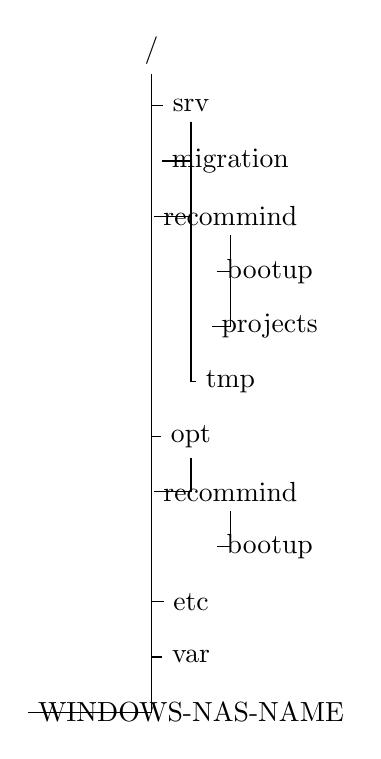
\begin{tikzpicture}[
		grow via three points={one child at (0.5,-0.7) and two children at (0.5,-0.7) and (0.5,-1.4)},
		edge from parent path={(\tikzparentnode.south) |- (\tikzchildnode.west)}]
		\node(root) {/}
			child { node {srv}
				child { node {migration}}
				child { node {recommind}
					child { node {bootup}}
					child { node {projects}}
				}
				child [missing] {}
				child [missing] {}
				child { node {tmp}}
			}
			child [missing] {}
			child [missing] {}
			child [missing] {}
			child [missing] {}
			child [missing] {}
			child { node {opt}
				child { node {recommind}
					child { node {bootup}}
				}
			}
			child [missing] {}
			child [missing] {}
			child { node {etc}}
			child { node {var}}
			child { node {WINDOWS-NAS-NAME}};
	\end{tikzpicture}
	
	The directories \emph{/srv/recommind}, \emph{/srv/migration} as well as the \emph{/WINDOWS-NAS-NAME} are shared between the Linux host and the docker container as mentioned in chapter \ref{p01:ch021} on page \pageref{p01:ch021} already.
	\section{Setting up CORE docker containers}
	In chapter \ref{p01:ch1} we mentioned the build pipeline. Now we describe the CORE installation procedure in more detail.
			\subsubsection{Docker image types}
			First we treat the different CORE docker image types and their responsibilities. The different docker image files are located at \emph{integration/docker} in the CORE repository:
						
			\tikzstyle{every node}=[draw=black,thick,anchor=west]
			\tikzstyle{selected}=[draw=red,fill=red!30]
			\tikzstyle{optional}=[dashed,fill=gray!50]
			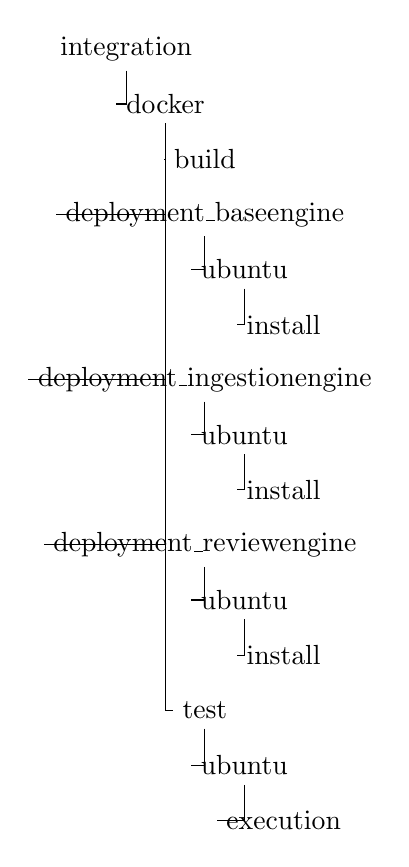
\begin{tikzpicture}[
				grow via three points={one child at (0.5,-0.7) and two children at (0.5,-0.7) and (0.5,-1.4)},
				edge from parent path={(\tikzparentnode.south) |- (\tikzchildnode.west)}]
				\node(root) {integration}
					child { node {docker}
						child { node {build}}
						child { node {deployment\_baseengine}
							child { node {ubuntu}
								child { node {install}}
							}
						}
						child [missing] {}
						child [missing] {}
						child { node {deployment\_ingestionengine}
							child { node {ubuntu}
								child { node {install}}
							}
						}
						child [missing] {}
						child [missing] {}
						child { node {deployment\_reviewengine}
							child { node {ubuntu}
								child { node {install}}
							}
						}
						child [missing] {}
						child [missing] {}
						child { node {test}
							child { node {ubuntu}
								child { node {execution}}
							}
						}
					};
			\end{tikzpicture}

			Those files are used to build the docker images. As there are dependencies between the different images we have to ensure that the necessary parent images exist before we build any image. As described in chapter \ref{p01:ch5} the \emph{build} docker image is based on \emph{build\_base} which doesn't live in the CORE repository. The same applies to \emph{deployment\_baseengine} which is a child of \emph{deployment\_base}. The CORE docker images have the following responsibility:
			\begin{description}\sloppy
				\item[build] The appropriate docker container is used for the build environment only. It provides the setup for the jenkins build job which performs the CORE java compile as part of the Ubuntu build.
				\item[deployment\_baseengine] This is a child image of \emph{deployment\_base}. Its parent is a base image for of all application specific docker containers like App server, CORE and Pgbouncer. Those containers usually contain java applications and have their own bootup logic which is implemented in python. Therefore the parent docker image file contains installation instructions for java, python and the required python modules. Furthermore \emph{deployment\_base} defines the bootup location \emph{/opt/recommind/bootup} where the bootup scripts can be found as well as a docker entrypoint in order to trigger those scripts after container startup.
				
				\emph{deployment\_baseengine} in turn is a parent of different CORE containers. The docker image file includes installation instructions in order to install the CORE zip. There are some installation scripts located at \emph{/integration/docker/deployment\_baseengine/ubuntu/install} which are copied into the docker container and triggered as part of the docker image build.
				\item[deployment\_ingestionengine] This is a child image of \emph{deployment\_baseengine}. Its install script copies the \emph{configuration.system.properties} file to the bootup source directory. This file contains the \emph{ingestion} role name which is consumed by the CORE bootup procedure.
				\item[deployment\_reviewengine] Same as mentioned in \emph{deployment\_ingestionengine} but we use the role \emph{reviewengine} and the install script installs the classic Axcelerate zip additionally.
				\item[test] This is a child image of \emph{deployment\_reviewengine}. It is used to run Ubuntu gate tests on the jenkins build machine. The \emph{execution} folder contains a script which takes the following arguments:
				\begin{itemize}
					\item --force\_run\_all: Optional flag to force the execution of all test suits even in case of failing suites.
					\item list of test suites: At least one gate test suit must be given. The paths are relative, e.g. \emph{gate/infrastructure/testsuite\_coreapi\_measures.xml}.
				\end{itemize}
				If any suite fails on the jenkins system, the \emph{mindserver-projects} folder will be archived and saved as \emph{mindserver-projects.zip} on \emph{laos} in an appropriate sub folder of \emph{.../CORE\_major\_minor/UbuntuGateTestLogs/build/distributions/test-output/...}. In addition we find a \emph{result.csv} file at this location which contains the failed suite names, the number of total tests per suite as well as the number of skipped and failed tests.
				
				Please note that the script consumes a \emph{TESTAGENT} zip file and the following environment variables:
				\begin{itemize}
					\item MINDSERVER\_HOME
					\item MINDSERVER\_PROJECTS
					\item JAVA\_HOME
					\item TEST\_VOLUME: The location where the \emph{test-output} folder will be created. Furthermore the script expects the \emph{TESTAGENT} zip file here.
				\end{itemize}
			\end{description}
			
			\subsubsection{The CORE bootup phases}
	\chapter{The new \texttt{bootloader}: An overview}\label{p01:ch04}
	\section{The bootloader architecture}
	\section{Host- and application-centric reliability}
	\section{Convinience functions in \texttt{lib}}
	\section{The boot phases}
		\subsection{The \texttt{common} role}
		\subsection{The \texttt{docker\_host} role}
		\subsection{The \texttt{batch\_asg} role}
		\subsection{The \texttt{master} role}
	\section{The shutdown phases}
	\chapter{The docker architecture}\label{p01:ch5}
	\section{A short introduction to docker}
		\subsection{What is docker}
		Docker is a technology to containerize software applications together with their dependencies into a complete environment and thus isolating them from other processes. As such the docker hosts environment does not need to be poluted by software installations and configurations. It makes it very easy to deploy a software as everything needed to run the software is contained within the container. From a technological point of view docker uses the Linux kernel techniques like cgroups to limit the set of resources the encapsulated environment is able to access.
		\subsection{Images and Containers}
		Before we can run containers containing our software we first need to build a docker image. From that image a container can be instantiated which then runs everything we described in the environment we configured during image creation.
		\subsection{Docker description files}
		To create an image we use a \emph{\dockerfile{}} which describes how our environment looks like. For example if we would like to run an ssh daemon within a docker container (although it might not has much sense as you only can login \emph{into} the container not the host) a minimal \dockerfile{} would look like this:
		\begin{listing}[H]
			\caption{A sample \dockerfile{}}
			\label{lst:p01:ch05:sample_dockerfile}
			\inputminted{text}{\relative{chapter_04/section_5.1.2/Dockerfile}}
		\end{listing}
		\begin{itemize}
			\item[FROM] The \mintinline{text}{FROM} instruction tells us on what image the new one is based on (we don't create images from scratch thus we don't need to deal with creating a ``root'' image). Here it is based on an image with a minimal ubuntu 16.04 environment. 
			\item[RUN] The next \mintinline{text}{RUN} statement executes the commands which follow the instruction during the image build process. Here we update the package list, install the latest fixes, install the openssh server and finally create the pid-file location for the ssh daemon. In the second \mintinline{text}{RUN} statement we change the password for \rootuser{} to be \rootuser{} (this is a lightweight example not accounting for security. Never ever do this; this description is based on a minimal example for creating a horneypot and for that purpose it was desired to make the break into the system for an intruder as easy as possible).
			\item[EXPOSE] This statement will ensure that the port following to the instruction is exposed to the docker host. Remember that docker is a container-technology which isolates the environment we encapsulate. By default this also means that the ports used within the container are not exposed to the outside world.
			\item[CMD] This statement defines the command which shall be executed once the we run the image. In our case here we want the ssh daemon to start.
		\end{itemize}

		\subsection{Repositories}
		A repository is a location or endpoint an image is put into. This can be local as well as a remote endpoint. For better organization images we can be tagged/labeled. If not specified the default tag ist \mintinline{text}{latest}.
		\subsection{The most relevant docker commands}
		The docker container system is very complex. However most of the time the set of commands you will need to deal with is small. The in our opinion most relevant commands will be described here.
			\subsubsection{\mintinline{text}{docker images}}
			\mintinline{text}{docker images} gives us just a list of every image in our system and looks like this:
			\begin{listing}[H]
				\caption{Output of docker images}
				\label{lst:p01:ch05:docker_images}
				\inputminted{text}{\relative{chapter_04/section_5.1.2/docker_images.lst}}
			\end{listing}
			Here we see a list of three images. Note the first two images do have two different tags namely latest and a convention we use in our docker base repositories (see section \ref{p01:ch05:docker_base_repos} for an explaination about the naming convention). But it is the same image what you can see if you take a look at the image id. 
			\subsection{\mintinline{text}{docker pull}}
			We use the combination of the repository and the tag to uniquely identify a specific docker image. For example the first image id \mintinline{text}{745551d6bb3} could be pulled by executing \mintinline{text}{docker pull recommind/deployment-base:latest}. Of course we would need access to the repository \mintinline{text}{recommind/deployment-base}. Here in our example we don't have a address schema in our repository name as it is a local repository. To get a more complete example of how to login and pull images from a remote target please see section \ref{p01:ch05:container_service_login}
			\subsubsection{\mintinline{text}{docker build} and \mintinline{text}{docker tag}}
			To create a docker image we use the \mintinline{text}{docker build} command. The minimum arguments required is a so called \emph{build context} on the assumption that the \dockerfile{} resides in current working directory. Otherwise the \dockerfile{} can be refered to by the \mintinline{text}{-f} option. The \emph{build context} defines the scope with in the filesystem which is available for access to the \mintinline{text}{docker build} process. Since we're able to place files from the host system into the docker image during image creation the \mintinline{text}{docker build} process needs access to them. And since the \mintinline{text}{docker build} process is already a container process we need to specify a location which can be mapped into this process to give it access to files which are needed during image creation. The build process does \emph{not} have access to the whole system.
			
			Lets assume our \dockerfile{} is the one from listing \ref{lst:p01:ch05:sample_dockerfile}. The following listing shows the command we could use to build the docker image. We omitted parts of the \mintinline{text}{apt-get} output as it is a lot:
			\begin{listing}[H]
				\caption{Output of docker build}
				\label{lst:p01:ch05:docker_build}
				\inputminted{text}{\relative{chapter_04/section_5.1.2/docker_build.lst}}
			\end{listing}
			We told the build process to use the current working directory as our build context (by specifying \mintinline{text}{.} as last parameter to the command). So the first thing the build process is doing is to scan the build context to get aware of everything in it. As there is only the \dockerfile{} the process tells us the size of that file (as this is the size of data residing within the build context). Then the build process just executes every statement in the \dockerfile{}. Every such statement defines a step to be executed. Every such execution modifies the intermediate docker image. Like a version control system this modification will be committed hence we gain a new intermediate container. Like vcs's docker is aware of what changes were already committed if one step failed for whatever reason we can fix it, build again and the docker process will recognize that it only needs to apply the steps which were not committed already.
			
			So lets take a look at the first step. The first step tells the build process what image we're going to modify. Here we refered the image by \mintinline{text}{ubuntu:16.04}. Taking a look at the docker images in listing \ref{lst:p01:ch05:docker_images} shows that this image has id \mintinline{text}{f753707788c5}. So the build process takes this as our base. It than spawns a container of this image with id \mintinline{text}{451e73b4d1a5} and executes the statement. The result is a modified environment which the build process commits yielding a new intermediate docker image with id \mintinline{text}{6fab3ba17962}. As we don't need the spawned container anymore it tells us that he's going to remove that intermediate container. This procedure will be repeated until the \dockerfile{} has been processed completely. The last commit then defines the id of our image:
			\begin{listing}[H]
				\caption{List of docker images after docker build}
				\label{lst:p01:ch05:list_images_after_build}
				\inputminted{text}{\relative{chapter_04/section_5.1.2/list_images_after_build.lst}}
			\end{listing}
			We notice two things. First the new image listed has the image id which was reported in the success message of the build process. And second that the repository as well as the tag is specified as \mintinline{text}{none}. The reason is that we did not tell the build process to put the new image into a repository and tag it. We can catch up on this by tagging the image explicitely:
			\begin{listing}[H]
				\caption{Tagging an image}
				\label{lst:p01:ch05:tag_image}
				\inputminted{text}{\relative{chapter_04/section_5.1.2/tag_image.lst}}
			\end{listing}
			It is of course possible to tell the \mintinline{text}{docker build} process to tag the created image directly by specifying \mintinline{text}{-t reposirotyname:tag} as parameter.
			\subsubsection{\mintinline{text}{docker run} and \mintinline{text}{docker ps}}
			To spawn a container out of an image we use the \mintinline{text}{docker run} command. The easiest format is just
			\mintinline{text}{docker run <image_id>}. However, remember that we specified in the \dockerfile{} that the command to be executed is to start the sshd daemon and if not specified otherwise the run process will start the container in \emph{attached} mode i.e. we're attached to the container. But since the daemon is no shell the command just don't return until the sshd terminates. Fortunately we can start the container in \emph{dettached} mode by specifying the \mintinline{text}{-d} option. The run command has a whole bunch of options. We will not discuss every option here. You can get a list of all options by executing \mintinline{text}{docker help run}.
			
			Now to see that our container started successfully we just list the docker container processes. Here is how the run and ps list looks like:
			\begin{listing}[H]
				\caption{Running an image}
				\label{lst:p01:ch05:run_image}
				\inputminted{text}{\relative{chapter_04/section_5.1.2/run_image.lst}}
			\end{listing}
			\subsubsection{\mintinline{text}{docker rm} and \mintinline{text}{docker rmi}}
			\subsubsection{\aws{} Container Service login}\label{p01:ch05:container_service_login}
%			For example we do use the docker service in \aws{}. The address scheme of the container service is \mintinline{text}{https://<accountnum>.dkr.ecr.us-east-1.amazonaws.com}. To be able to pull and push images to that repository we would use \mintinline{text}{docker login -p password -u username https://<accountnum>.dkr.ecr.us-east-1.amazonaws.com}
	\section{The base docker mercurial repositories}\label{p01:ch05:docker_base_repos}
		\subsection{Naming conventions for docker repository names}
		\subsection{The \texttt{foundation} repository}
		\subsection{The \texttt{build\_base} repository}
		\subsection{The \texttt{deployment\_base} repository}
	\section{The docker images in cg}
		\subsection{The \texttt{build} repository}
		\subsection{The \texttt{deployment\_baseengine} repository}
		\subsection{The \texttt{deployment\_ingestionengine} repository}
		\subsection{The \texttt{deployment\_reviewengine} repository}
		\subsection{The \texttt{test} repository}
		\subsection{The cg docker gradle tasks}
	\chapter{The \texttt{AxceleratePod} repository}
	\section{Orchestrating a Linux machine}
	\section{The bridge between orchestratiion and dev: \texttt{ec2\_impl.py}}
	\section{Entrypoint: \texttt{userdata}}
		\subsection{The salt configuration}
		\subsection{The bootloader hotfix}
		\subsection{The pip hotfix}
		\subsection{The bootloader startup}
	\section{The host instance bootloader configuration}
	\section{The container bootloader configuration}
	\renewcommand\relativepath{c:/documentation/recomlinarch/part_02/}
	\part{POD orchestration and testing}
	\chapter{\pod{} Orchestration}
	\section{Introduction}
	Each customer environment is organized in so called \pod{}s. A \pod{} is roughly a VPN where all the servers are located which are configured as the customer needs it. To create a \pod{} we need to login to a server which serves a specific role: The orchestration server. The orchestration server has installed a couple of (partially self-developed) software packages which we use to create, extend and terminate \pod{}s.
	\section{Orchestration Server}
	We do have several orchestration server. To get a list login to the \awsc{} and navigate to the service \emph{Instances}. Then filter the instances by \emph{VADORC}. Now you get a list of all orchestration server available. There are some orchestration server which are used by specific people and before using them you should contact at least those people and ask if the server can be used for your needs. This is very important as we do have a big drawback: Every orchestration server clones the orchestration repository and you typically work directly inside this repository and you need to do so as user \emph{root}. The consequence is that actions of multiple users at the same time are extremely dangerous. For example if user \mintinline{shell}{A} upgrades a \pod{} and user \mintinline{shell}{B} changes the branch of the orchestration repository to a different one of \mintinline{shell}{A} you can destroy \mintinline{shell}{A}'s \pod{} as his commands will be based on the changed repository. So it is crucial to make sure that no other orchestration process or user is working on that machine at the same time.

           % FIXME: complete the list
           Figure \ref{tab:p03:ch01:overview_orch_servers} shows a list of orchestration servers together the person or team they're reserved for and whom can be asked if the server is free to use.
           \begin{table}[h]
             \center
             \caption{Overview of the orchestration servers and responsibility}
             \begin{tabular}{| l | l | p{5cm} |}
               \hline
               \textbf{Instancename} & \textbf{Responsibility} & \textbf{Note} \\ \hline
               \vadorc{05} & Benjamin Schiborr & Usually free to use. If unsure you also may ask jsr \\ \hline
               \vadorc{06} & Nate & Usually used by Nate. But might be free to use for us too. Ask jsr if unsure. \\ \hline
               \vadorc{07} & Team TS & \\ \hline
             \end{tabular}
             \label{tab:p03:ch01:overview_orch_servers}
           \end{table}
	\section{Working with the orchestration server}
             \subsection{Login to the orchestration server}
             Before we come to the filesystem layout and how we setup the orchestration server to be operational and start working we need to login to the orchestration server. To to so we need to use one of our jump hosts as the orchestration servers themselves are not accessible from outside. To be able to login into a jump host you have to have a working 2FA setup for your personal use.
             Pick one of the jump hosts of the following list and use \rdp{} to login to the server. Remember to use the appropriate credentials depending on whether you are going to do your work in the production or the development environment.

           Once your on the jump host start putty to login to the orchestration server of your choice. If the orchestration server of your choice is not already saved at your putty profile create it and make sure that you use the appropriate private key for login. The available private keys can be found in the putty's installation directory. The one you need to use is the \emph{\awsstddevkey}. You can use this key in putty by loading your session and navigate to \emph{Connection $\rightarrow$ SSH $\rightarrow$ Auth $\rightarrow$ Keys} and select the key from the putty installation directory. Once done save the session and start to login.
           
		\subsection{Setup the orchestration server}
             Before we can start using the orchestration scripts we need to ensure that the orchestration docker service is running. The docker container for the orchestration service has the name \emph{orch}. Check that the orchestration service is running by executing the following command:
         	\begin{minted}{shell}
> docker ps | grep orch
dc92f331d1ce        orchestration:latest   "/usr/local/bin/super"   
    32 hours ago        Up 32 hours         ...   orch
           	\end{minted}
           If it is not running we need to start the orchestration docker service first. Before you do so ensure that you are \rootuser{}. You can request to get \rootuser{} by using your \emph{rmdevcloud2} credentials by executing the command
             \begin{minted}{shell}
user@rmdevcloud2.int@vadorc05:~$ sudo su
[sudo] password for user@rmdevcloud2.int:
root@vadorc05 /home/user@rmdevcloud2.int >
           \end{minted}
           Once done it is recommended to change the directory to \mintinline{shell}{/srv/orchestration/}. Here we find the orchestration base directory of the orchestration repository. It is the root where the base actions take place like changing the orchestration to the code base which you might need for your further actions. For example if you want to create a new \pod{} with a specific version you need to change the orchestration code base to exactly this version too.
           
           The next step would be to start the orchestration docker service with the command
           \begin{minted}{shell}
root@vadorc05 /home/user@rmdevcloud2.int > ./docker/initialize_docker.sh
           \end{minted}
           Wait for the docker container to come up. Once the command finishes we can test that the orchestration docker service works properly by executing
           \begin{minted}{shell}
root@vadorc05 /home/user@rmdevcloud2.int > salt '*' test.ping
           \end{minted}
           and verifying that the result does \emph{not} says that the command timed out. If you get a list of servers or the result that nothing could be found everything is ok even though if single servers does not respond to the ping (which might be expected as not every server is running).

           If on the other hand the ping command tells you it timed out the orchestration docker service initialization failed (at the present time this can happen; we don't know why. There is ongoing work to stabalize this) and you need to repeat the step setting up the service by executing
           \begin{minted}{shell}
root@vadorc05 ... > docker stop orch && docker rm orch && \
  ./docker/initialize_docker.sh
           \end{minted}
           Once again use the salt-command to check that the orchestraton docker service does work.

	\section{The relation of the orchestration and axceleratepod repository}
	Before we go forward explaining how to create or modify a \pod{} we want to address the relationship between the orchestration and axceleratepod repository. It is important to know that the orchestration repository actually does not contain the orchestrating code. It is more a facet which serves as a layer for configuration and which \emph{feeds} a specific version of the implementation of axceleratepod to orchestrate a \pod{}. As such the axceleratepod can be seen as a orchestration library which is used by the code orchestration code to create or modify a \pod{} with respect to a given configuration. It also specifies the software stack - i.e. the version of cg, ng etc. pp. - which is to be used within the pod.
	
	Nevertheless it does not suffice to just exchange the axceleratepod version. Also the orchestration code base needs to be conform to the axceleratepod version which is going to be used to orchestrate a \pod{}. The version control system to use here is \git{}. The branches for a release \mintinline{shell}{R} has the format \mintinline{shell}{releases/R} where \mintinline{shell}{R} is the software version to run inside the \pod{} (like \mintinline{shell}{5_10}).
	
	Before you change the branch of the orchestration repository to begin your work it is \emph{very} important to check first whether there is another user on the system working. As you need to be \rootuser{} on the system and since working with the orchestration means you're working directly on the orchestration repository system wide changing the branch of the repository while there is some ongoing orchestration process could result in a damanged \pod{}!
	
	Unfortunately it can be tedious to find out who is actually working on the system. You can try \mintinline{shell}{who} or \mintinline{shell}{users} to request which users are on the system. However if someone did not use his domain user login and did the login using the ubuntu user there is no direct way to determine whom is online. If unsure take a look at table  \ref{tab:p03:ch01:overview_orch_servers} and contact the contact person listet there.
	
	Once it is clear that you can use the server (if not you need to find another server which is free to use) you need to assume that the person who used the server previously did not left the repository in a clean state. To check if there are uncommitted changes type
	\mintinline{shell}{git status}. If there are uncommitted changes you can just stash them (as we assume that you are free to use the orchestration server) using \mintinline{shell}{git stash}. Once done change the branch to the one you need like
           \begin{minted}{shell}
root@vadorc05 ... (git)-[releases/5_10] > git stash
Saved working directory and index state WIP on releases/5_10: bac6908 
  Changes small.yaml.
HEAD is now at bac6908 Changes small.yaml.
root@vadorc05 ... (git)-[releases/5_10] > git checkout your_branch
Switched to branch `your_branch'
root@vadorc05 ... (git)-[your_branch] >
           \end{minted}
	
	\section{Creating a \pod{}}
	We assume that our working directory is \mintinline{shell}{/srv/orchestration} and that we're \rootuser{} and that the server is free to use. If we know the software version we want to deploy the only thing left is to specify how the \pod{} is going look like, i.e. which servers and how many of them we want to instantiate. To specify this there is a yaml-configuration file which lists each server type we want to instantiate and how many of those servers we want to have.
	
	There are planty of those files. But to keep it simple and as long as we cannot just specify an own file (which is in progress at the present time) we just need to edit \mintinline{shell}{/srv/orchestration/puppet/environments/development/hiera/06_size/small.yaml} an example of the is given in listing \ref{lst:p03:ch01:orchestration}
	\begin{listing}[H]
		\caption{A sample pod instance description}
		\label{lst:p03:ch01:orchestration}
		\inputminted{yaml}{\relative{chapter_00/section_1.4/pod_instance_description.yaml}}
	\end{listing}
	As you can see here our pod would consist of one master-service server, one ingestion server as well as one axcelerate server based on Linux as well as one nas and database server. We could list every other instance type with count equal to $0$ but we kept the file as small as possible. Table \ref{tab:p03:ch01:instance_types} gives an overview over every instance type you might want to specify here:
	\begin{table}[h]
         \center
         \caption{Available instance types}
         \begin{tabular}{| l | l | l |}
           \hline
           \textbf{Instance type} & \textbf{Remark} \\ \hline
           master & The master service instance. Platform: Windows \\ \hline
           batch\_asg & A batch auto scaling instance \\ \hline
           crawler & A Windows based crawler instance \\ \hline
           app & An instance for service and web tier \\ \hline
           ingestion & A Windows based ingestion instance \\ \hline
           ingestion\_linux & A Linux based ingestion instance \\ \hline
           axcelerate & A Windows based axcelerate instance \\ \hline
           axcelerate\_linux & A Linux based axcelerate instance \\ \hline
           nas & A Windows file sharing instance \\ \hline
           admin & A Windows based instance holding the admin application \\ \hline
           db & NG db service as \aws{} service \\ \hline
         \end{tabular}
         \label{tab:p03:ch01:instance_types}
      \end{table}
	
	Now configure you're \pod{} as you need it. Once finished you start creating the \pod{} by executing
	\begin{minted}{shell}
root@vadorc05 ... (git)-[releases/5_10] > orchestration create 
  -T pod_env -I tenant -P pod_id -R region -A account_number --costcenter 
  user@opentext.com --version version
	\end{minted}
	where the arguments do have the following meaning:
	\begin{description}
		\item[-T] Specifies the \emph{environment} of the \pod{}. See table \ref{tab:p03:ch01:pod_envs} for a list of available arguments.
		\item[-I] Specifies the \emph{tenant id} for which the \pod{} is to be created. Note: You cannot choose a abitrary value here. The tenant id needs to be existent in the launchpad. If you need a new one someone from Infrastructure or QA Tooling might be able to help you creating a new one.
		\item[-P] Specifies the \emph{\pod{} id}. If you need multiple \pod{}s for one tenant you can enumerate the \pod{}s through this parameter.
		\item[-R] Specifies the \aws{} region where the \pod{} is to be created. Usually it is \emph{us-east-1}.
		\item[-A] Specifies the \aws{} account which is used to create the \pod{}. See table \ref{tab:p03:ch01:aws_account_nums} for a list of accounts which can be used here.
		\item[--costcenter] Specifies the cost center. Usually the email of the person or team who created/modified the \pod{}.
		\item[--version] Specifies the product version which shall be deployed onto the instances of the \pod{}. The version you can specify here is the \axceleratepod{} version which contains the software distribution (core-version, ng-version, ami-id to use for the instances etc. pp.) and needs to be existent. Usually you will choose a released software version like in the example (we use the ng-versioning here; not core-versioning). How this relates to custom version testing see chapter \ref{p03:ch02:pod_testing}
	\end{description}
	\begin{table}[h]
         \center
         \caption{\aws{} Environment parameters}
         \begin{tabular}{| l | l |}
           \hline
           \textbf{Paramter name} & \textbf{Remark} \\ \hline
           development & \\ \hline
           staging & Technically this is a production environment \\ \hline
           production & \\ \hline
         \end{tabular}
         \label{tab:p03:ch01:pod_envs}
      \end{table}
	\begin{table}[h]
         \center
         \caption{\aws{} Account numbers}
         \begin{tabular}{| l | l | l |}
           \hline
           \textbf{Account number} & \textbf{Target} & \textbf{Domain to use to login into instances} \\ \hline
           710991980648 & Development account  & rmdevcloud2.int \\ \hline
           569599628740 & Production account &  rmcloud; needs 2FA\\ \hline
         \end{tabular}
         \label{tab:p03:ch01:aws_account_nums}
      \end{table}
	
	\section{Adding an instance to a \pod{}}
	Adding a new instance uses almost the same parameters like creating a pod. There is one more parameter \mintinline{shell}{--scale_role}
	which expects an instance type as its argument which we want to add to the \pod{}:
	\begin{minted}{shell}
root@vadorc05 ... (git)-[releases/5_10] > orchestration add --scale_role
   instance_type -I tenant -P pod_id -R region -A account_number 
   --costcenter user@opentext.com --version version
	\end{minted}
	The instance type is one of the table \ref{tab:p03:ch01:instance_types}.

	\section{Terminating a \pod{}}
	We can terminate a whole \pod{} by using the command
	\begin{minted}{shell}
root@vadorc05 ... (git)-[releases/5_10] > orchestration terminate 
  -I tenant -P pod_id -R region -A account_number --costcenter 
  user@opentext.com --version version
	\end{minted}
	
	\section{Start and stop a \pod{}}
	To start and stop the services running on the instances of a \pod{} you can use the following command:
	\begin{minted}{shell}
root@vadorc05 ... (git)-[releases/5_10] > orchestration start/stop 
  -I tenant -P pod_id -R region -A account_number --costcenter 
  user@opentext.com --version version
	\end{minted}
	If you stop a \pod{} you can use the optional parameter \mintinline{shell}{--stop_instances} to also stop the instances as well.

%	\begin{description}
%		\item[clone]
%		\item[recovery]
%		\item[snapshot]
%		\item[update]
%		\item[tag]
%		\item[rollback]
%		\item[reinstantiate]
%		\item[configure]
%		\item[state]
%		\item[migrate]
%		\item[patch]
%	\end{description}

	\chapter{\pod{} Testing}\label{p03:ch02:pod_testing}
	\section{\axceleratepod{} changes}
	The \axceleratepod{} repository contains the implementation of the orchestration feature set, i.e. everything which is needed to manage pods (creating, extending, upgrading, migrating, terminating, etc. pp.). It also contains the part of our docker deployment infrastructure which is responsible to create every configuration needed by the docker host as well as the engine/app container and batch asg instances. Here we do not go into detail on the repositories layout but how to test changes of the repository.
	
		\subsection{Creating a new \axceleratepod{} version}
		For the sake of example lets assume we have some changes on some templates of the userdata and we want to do some testing that those changes are correctly reflected in the deployment process, i.e. using the orchestration process to create or modify a \pod{}. Lets furthermore assume we made our changes in some branch $B$ and we just pushed the changes.
		
		Before we can reference the \axceleratepod{} version based on $B$ we first need to create a new version of \axceleratepod{}. In this step the \axceleratepod{} version based on $B$ will be build, zipped and uploaded to S3 such that the orchestration server has access to it and hence is able to use it as the underlying implementation of the changed orchestration feature set.
		
		To do we open up the webpage
		\begin{center}
			http://rm-jenkins/job/create_pod_version_default/
		\end{center}
		perform a login using our credentials and navigate to \emph{Build with Parameters} side using the same titled navigation link to the left. Fill in $B$ for the textfield to the right of the \emph{branch} label and keep the other options as is. Hit the \emph{Build} button and wait until the \axceleratepod{} creation has been done. You can repeat those steps as often as you need it. For instance if you do need to change more on your branch. The concrete \axceleratepod{} version is labeled
		\begin{center}
			$B$-$N$
		\end{center}
		where $N$ is a build number which is increased on each \axceleratepod{} creation you perform.
		
		\subsection{Using the new \axceleratepod{} version}
		Now as we created a new \axceleratepod{} version we can use it in our orchestration steps. For the details on how to work with the orchestration server please refer to section \ref{p03:ch01:working_with_orch_servers}. In every sub-command of the orchestration script which supports the \mintinline{-version} option (like \mintinline{create}) we can now pass $B$ as \axceleratepod{} version to use. Note that we do not specify the build version here. As default the latest version of $B$ is being used by the orchestration tool. If we want to use a specific version $N$ we can tell the tool so by specifying $N$ using the command line option \mintinline{--minor_version N}. Anything done by the orchestration steps will now be based on the \axceleratepod{} version $B$-$N$.
	\section{Bootloader changes}
	Sometimes we need to test changes to the bootloader as well. There are two standard scenarios here: changes to the bootloader phases regarding the docker host and the once which reside within the deployed docker container. 
		\subsection{Docker host specific changes}
		The easiest to test are bootloader changes to phases which resides in the docker host bootloader installation. For such changes a \emph{hotfix} mechanism has been implemented which works as follows: The userdata script on a Linux host looks at some predefined location for a custom bootloader. If such a bootloader could be found it is downloaded and the bootloader already installed on the Linux host will be replaced by the userdata with the new bootloader just before the bootloader is executed.
		\subsection{CG/NG specific changes}
		\subsection{Special handling of changes for batch asg}
	\section{CG changes}
		\subsection{Promote new docker images using jenkins}
		\subsection{Push docker images manually}
	\listoflistings
\end{document}
